\usetikzlibrary{shadows,arrows.meta,positioning,backgrounds,fit}

\usetikzlibrary{shapes}
\usetikzlibrary{shapes.callouts}
\usetikzlibrary{shapes.geometric}

\usetikzlibrary{arrows}
\usetikzlibrary{decorations}
\usetikzlibrary{snakes}
\usetikzlibrary{calc}
\usetikzlibrary{patterns}

\usetikzlibrary{matrix,patterns,chains}
\usetikzlibrary{arrows,automata}
\usetikzlibrary{mindmap,trees}
\usetikzlibrary{shapes,snakes}
\usetikzlibrary{circuits.logic.US}
\usetikzlibrary{calc,intersections}

\tikzset{input/.style=coordinate}
\tikzset{output/.style=coordinate}
\tikzset{
  % coord node style is used for placing corners of connecting lines
  coord/.style={coordinate, on chain, on grid, node distance=6mm and 25mm},
  test/.style={draw, diamond, aspect=2, text width=5em},
  block/.style={draw, rectangle,
  minimum height=3em,
  minimum width=7em}}
  
\tikzset{pinstyle/.style={pin edge={to-,thin,black}}}

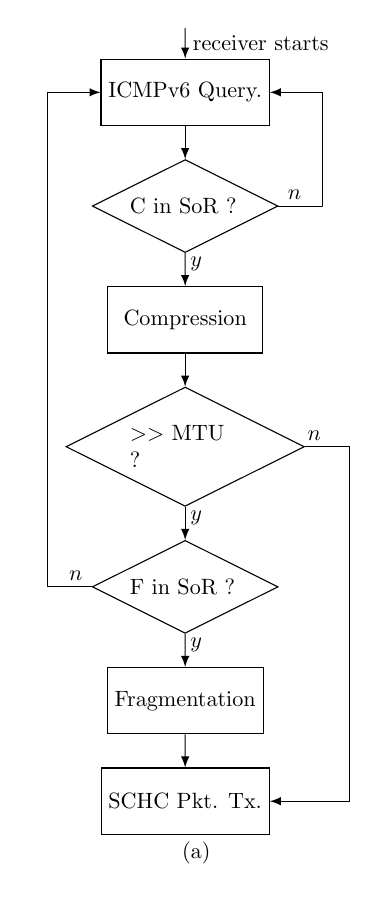
\begin{tikzpicture}[%auto, node distance=2cm,>=latex',
    xscale=0.8,
    yscale=0.8,
    transform shape,
    >=latex,              % Nice arrows; your taste may be different
    start chain=going below,    % General flow is top-to-bottom
    node distance=6mm and 60mm, % Global setup of box spacing
    every join/.style={norm},   % Default linetype for connecting boxes
    ]

\node (input) [input] {\textit{start}};

\node (start) [below right] at (input.south) {receiver starts};

\node (rx) [block, below, align=left] at (start.south west)
{ICMPv6 Query.};

\node (selectc) [test, below, align=left, yshift=-1.5em] at (rx.south)
{C in SoR ?};

\node [coord, right=of selectc] (non)  {}; %coordinates for the non path

\path (selectc.east) to node [near start, yshift = 0.5em] {$n$} (non); 
\path (selectc.south) to node [near start, xshift = 0.5em, yshift = -0.5em] {$y$} (selectc);

\node (comp) [block, below, align=left, yshift=-1.5em] at (selectc.south)
{Compression};

\node (selectmtu) [test, below, align=left, yshift=-1.5em] at (comp.south)
{$>>$ MTU ?};
\node [coord, right=of selectmtu] (non1)  {}; %coordinates for the non path
\path (selectmtu.east) to node [near start, yshift = 0.5em] {$n$} (non1); 
\path (selectmtu.south) to node [near start, xshift = 0.5em, yshift = -0.5em] {$y$} (selectmtu);

\node (selectf) [test, below, align=left, yshift=-1.5em] at (selectmtu.south)
{F in SoR ?};

\node [coord, left=of selectf] (non2)  {}; %coordinates for the non path
\path (selectf.west) to node [near start, yshift = 0.5em] {$n$} (non2); 
\path (selectf.south) to node [near start, xshift = 0.5em, yshift = -0.5em] {$y$} (selectf);


\node (frag) [block, below, align=left, yshift=-1.5em] at (selectf.south)
{Fragmentation};

\node (tx) [block, below, align=left, yshift=-1.5em] at (frag.south)
{SCHC Pkt. Tx.};

\draw [->] (input) --  (rx);    
\draw [->] (rx.south) -- (selectc);
\draw [->] (selectc.south) --  (comp);
\draw [->] (comp.south) --  (selectmtu);
\draw [->] (selectmtu.south) --  (selectf);
\draw [->] (selectf.south) --  (frag);
\draw [->] (frag.south) --  (tx);

\coordinate (fb) at ($(selectc.east)+(2em,0)$); %fb -- feedback
\draw [->] (selectc.east) -| (fb) |- (rx.east);

\coordinate (fb1) at ($(selectf.west)-(2em,0)$); %fb -- feedback
\draw [->] (selectf.west) -| (fb1) |- (rx.west);

\coordinate (fb) at ($(selectmtu.east)+(2em,0)$); %fb -- feedback
\draw [->] (selectmtu.east) -| (fb) |- (tx.east);

\path (tx.south) to node [near start, xshift = 0.5em, yshift = -0.8em] {(a)} (tx);


%\coordinate (fb) at ($(jam.west)+(-2em,0)$); %fb -- feedback
%\draw [->] (output) -| (fb) |- (loop.west);
%\coordinate (fb1) at ($(select.east)+(2em,0)$); %fb -- feedback
%\draw [->] (select.east) -| (fb1) |- (loop.east);

%\node (label) [below, yshift = - 0.3em] at (jam.south) {(a)};

\end{tikzpicture}